\documentclass{article}

\usepackage[utf8]{inputenc}
\usepackage[margin=1in]{geometry}
\usepackage[colorlinks=true, pdfborder={0 0 0}]{hyperref} 
\usepackage{microtype}
\usepackage{amsfonts}
\usepackage{amssymb}
\usepackage{graphicx}
\usepackage{subfig}
\usepackage{float}
\usepackage{siunitx}
\usepackage{listings}
\setcounter{topnumber}{8}
\setcounter{bottomnumber}{8}
\setcounter{totalnumber}{8}
\usepackage{arydshln}
\usepackage[framemethod=tikz]{mdframed}
\usepackage{minted}
\usepackage{empheq}
\usepackage{nicematrix}
\usepackage{titlesec}
\usepackage{multicol}

\usepackage[sorting=nty]{biblatex}
\addbibresource{sources.bib}

\hypersetup{
    colorlinks=true,
    citecolor=black,
    linkcolor=black,
    urlcolor=black
}

\let\oldhyperlink\hyperlink
\renewcommand{\hyperlink}[2]{\oldhyperlink{#1}{\textbf{#2}}}

\let\oldcite\cite
\renewcommand{\cite}[1]{\textbf{\oldcite{#1}}}

\setlength{\parindent}{0cm}
\setlength{\leftskip}{0cm}

\usepackage{amsmath}
% For annet format på formler:
% \usepackage[fleqn]{amsmath}
% \setlength{\mathindent}{0cm}

\lstset{
  language=Python,
  basicstyle=\footnotesize\ttfamily,
  %keywordstyle=\color{blue},
  %commentstyle=\color{green},
  %stringstyle=\color{red},
  numbers=left,
  numberstyle=\tiny,
  numbersep=5pt,
  breaklines=true,
  showstringspaces=false,
  xleftmargin=.25in,
  xrightmargin=.25in
}

\definecolor{barcolor}{rgb}{0,0,0}
\renewenvironment{leftbar}[1][\hsize]{
    \def\FrameCommand{{\color{barcolor}\vrule width 0.5pt \hspace{10pt}}}
    \MakeFramed{\hsize#1 \advance\hsize-\width \FrameRestore}
}{\endMakeFramed}

\titleformat{name=\section,numberless}[block]
  {\normalfont\Large\bfseries}
  {\llap{\rule[0ex]{0.6em}{0.6em}\hspace{1.8em}}}{0em}{\titlerule\\[.8ex]}{}

\renewcommand\thefootnote{\textcolor{black}{\arabic{footnote}}}
\renewcommand{\footnoterule}{}

\newcommand{\explain}[2]{\underbrace{#1}_{\parbox{\widthof{\ensuremath{#1}}}{\footnotesize\centering #2}}}
\usepackage{nicematrix}

\setlength{\parskip}{0.15cm}

\begin{document}

\begin{center}
    \textbf{\LARGE REINFORCEMENT LEARNING}

    %\rule{4cm}{1pt}
    \vspace{0.2cm}

    Hallvard Høyland Lavik

    2024

\end{center}

\section*{Motivation}

Reinforcement learning is a powerful approach within machine learning where an artificial neural network (hereafter "agent") learns to interact with an environment. These interactions result in either an instantaneous or delayed "reward" which incentivize the agent to learn the optimal actions with respect to different "states" within the environment.

Initially, an agent starts with no knowledge of the environment and must learn through trial and error which actions lead to positive rewards. This learning process involves adjusting the weights of the agent over many iterations to improve performance. In cases where the rewards are significantly delayed, this learning process may be challenging – as the agent is unable to determine which of its actions led to the reward. An example of extremely delayed reward is OpenAIs work on mastering Minecraft. They had a goal for their agent to obtain diamond tools, which "usually takes proficient humans over 20 minutes (24,000 actions)". They achieved this through sequentially rewarding the agent based on the progress it made, thus providing it with a more immediate reward based on its actions. \cite{Minecraft}

\section*{Methods}

Reinforcement agents aim to execute actions within an environment that result in the highest rewards. The term "reinforcement" is used because the agent's actions are influenced by its past experiences. Optimal behavior can be achieved through various reinforcement learning techniques, which are typically categorized into two main types: policy–based and value–based approaches.

A policy is a strategy that maps states to actions with the aim of maximizing future rewards. It is often represented as a probability distribution over the possible actions. On the other hand, the term "value" in value–based approaches refers to the mapping from states to the expected future rewards; it predicts the future reward for each action given an observed state.

Therefore, an agent can either learn to have confidence in its actions (policy–based) or try to estimate the expected value of being in a state (value–based). While the methods differ slightly, both aim to maximize future rewards.

\subsection*{\normalsize ON– AND OFF–POLICY LEARNING}
\begin{leftbar}
    Reinforcement learning algorithms can be further categorized into on–policy and off–policy methods. The distinction between these two lies in the way the agent's learning is updated.

    On–policy methods, such as policy–based approaches, involve the agent determining actions based on its current policy. The policy is then updated according to the reward received from the chosen action.

    Off–policy methods, on the other hand, involve the use of two separate policies: one for exploration and another for learning. An example of this is Q–learning. In Q–learning, the agent's network (Q) and the target network (Q–hat) are independent when calculating the loss, making it an off–policy approach.
\end{leftbar}
\subsection*{\normalsize POLICY–BASED APPROACH}
\begin{leftbar}
    Denoted as $\pi(a|s)$, the policy of an agent is the certainty of an actions $a$ will yield the highest possible future reward, given a state $s$. When the agent performs the most probable action, it observes the new state and is given a reward (assuming an immediate reward is given). Therefore, in a policy–based approach, finding the optimal policy (denoted as $\pi^\star (a|s)$) which maximizes the expected future rewards given the current state is what the agent leans to do. \cite{HF-approaches}

    \hypertarget{sec:policy-based-approach}{}
    \subsubsection*{POLICY–BASED GRADIENT}

    In a policy–based gradient approach, the performance of the agent is optimized based on the probability distribution of the possible actions given a state with respect to its parameters ($\pi(a|s)_\theta$). This optimization is based on the agent's experience in an on–policy manner, in order to obtain a gradient which then directly influence the parameters. \cite{HF-policy} While there are various approaches in determining the gradients, a modified version of the REINFORCE algorithm is implemented as:

    \fbox{
        \begin{minipage}{\textwidth}
            \begin{itemize}
                \item[] initialize agent
                \item[] \textbf{for} game \textbf{do}
                \item[] \begin{itemize}
                    \item[] create empty memory
                    \item[] observe initial state
                    \item[] \textbf{while} alive \textbf{do}
                    \item[] \begin{itemize}
                        \item[] forward propagate state through agent to obtain action probabilities
                        \item[] select action based on random weighted choice
                        \item[] execute chosen action
                        \item[] observe next state reward and mortality
                        \item[] store reward and logarithm of chosen action probability in memory
                    \end{itemize}
                    \item[] \textbf{end while}
                    \item[] calculate discounted rewards $R'$ based on memory
                    \item[] calculate policy gradient $G$ based on memory and $R'$
                    \item[] update agent parameters with respect to gradient
                \end{itemize}
                \item[] \textbf{end for} \hfill Modifed from Yoon \cite{REINFORCE}
            \end{itemize}
        \end{minipage}
    }

    Where the expected future reward $R_i$ for each time step $i \in [0, N]$ is calculated as:

    \begin{equation}
        \begin{split}
            R_i &= r_i + \gamma R_{i+1} \qquad \qquad 0 < \gamma < 1 \\
            R'_i &= (R_i - \mu_R) / \sigma_R
        \end{split} \label{eq:reward}.
    \end{equation}

    Here, $r_i$ is the reward at time step $i$, and $\gamma$ is the discount factor. The expected future rewards are calculated backwards, as $R_{N+1} = 0 \Rightarrow R_N = r_N$. These expected rewards are discounted, such that the rewards far into the future are worth less than instantaneous rewards. The expected rewards are then standardized.

    The policy gradient $G_i$ at each time step $i$ is calculated as:

    \begin{equation}
        G_i = - \log \left[ \pi(a_i|s_i) \right] \times R'_i \qquad \Rightarrow \qquad G = \sum_{i}^N G_i
    \end{equation}

    where $\pi(a_i|s_i)$ is the probability of taking the chosen action $a_i$ given state $s_i$ (\textit{i.e.}, $\max_{a} \pi (a|s_i)$). The overall gradient, $G$, is the sum of these individual gradients $G_i$.

\end{leftbar}
\subsection*{\normalsize VALUE–BASED APPROACH}
\begin{leftbar}
    In contrast to the \hyperlink{sec:policy-based-approach}{policy–based gradient approach} which outputs a probability distribution across the possible actions, the value–based approach predicts a Q-value (representing the expected future rewards) related to each possible action. \cite{HF-value}

    \hypertarget{sec:value-based-approach}{}
    \subsubsection*{Q–LEARNING}

    In order to learn optimal policy in an environment, a Q-learning agent learns to associate each state with expected rewards for each possible actions. The expected values for the states can thus be calculated through the state-value function (\textit{i.e.}, the Bellman equation):

    \begin{equation}
        \begin{split}
            V_\pi (s) &= E_\pi \left[ R'_{t+1} + \gamma V_\pi (S_{t+1}) | S_t = s \right] \\
             &= R'_t + \gamma \sum_{i=t+2}^T R'_i
        \end{split}
        \label{eq:value-function}.
    \end{equation}

    Here, $V_\pi (s)$ represents the value of state s under policy $\pi$, $E_\pi$ the expected: immediate reward $R'_{t+1}$ (see Equation \eqref{eq:reward}) plus the discount factor $\gamma$ times the value of the next state $V_\pi (S_{t+1})$. This equals the expected future rewards from $t$, given that the agent is at state s. \cite{HF-bellman} \cite{Q-traditional} \cite{Technical-Q-learning}

    The Bellman Optimality Equation for the Q–value (action–value function) can thus be derived from the state–value function \eqref{eq:value-function}:

    \begin{equation}
        Q(S_t, A_t) = E \left[ R_{t+1} + \gamma \times \max_a Q(S_{t+1}, a) \right]
        \label{eq:q-value}
    \end{equation}

    which yields the optimal Q–value for the given state and action following the optimal policy thereafter. This equation is the sum of the immediate reward and the discounted maximum expected reward for the next state, and therefore represents the value (\textit{i.e.}, reward) of taking the action. \cite{Q-intro} \cite{Human-level} \cite{Technical-Q-learning}

    Equation \eqref{eq:q-value} can thus be rewritten to encapsulate the Q-learning update rule:

    \begin{equation}
        Q(S_t, A_t) = Q(S_{t-1}, A_{t-1}) + \alpha \left[ R_{t+1} + \gamma \times \max_a Q(S_t, a) - Q(S_{t-1}, A_{t-1}) \right] \label{eq:q-star-traditional},
    \end{equation}

    where $\alpha$ is the learning rate of the agent \cite{Q-deep} \cite{Human-level}. This equation updates the Q-value for the state-action pair $(S_{t-1}, A_{t-1})$ based on the immediate reward $R_{t+1}$ and the maximum Q-value for the next state $S_t$, discounted by the factor $\gamma$.

    In traditional Q–learning, these values are stored in a table which thus contains all optimal actions for each given state. However, for environments with many and/or continuous actions and states this approach is not as efficient.

    \subsubsection*{DEEP Q–LEARNING}

    In deep Q–learning, the optimal Q–value is approximated through the agent instead of obtaining it from the Q-table – therefore the Q-table can be discarded, as all information is stored within the agent parameters.

    The parameters of the agent are updated in an off–policy manner with respect to a loss which is the difference between the predicted Q–value and a target Q–value, performing gradient descent with respect to this. \cite{Q-deep} Equation \eqref{eq:q-star-traditional} can therefore be modified and rewritten:

    \begin{equation*}
        \text{loss} = \explain{Q(R_t, a | \theta)}{\text{Q–predicted}} - \explain{R_{t+1} + \gamma \max_a \Hat{Q}(S_{t+1}, a | \Hat{\theta})}{\text{Q–target}}
    \end{equation*}

    Here, $Q(R_t, a | \theta)$ is the previously predicted Q-value for taking action $a$ at state $R_t$ given the parameters $\theta$, $R_{t+1}$ the immediate reward after taking action $a$ at time $t$, $\gamma$ is the discount factor, $\Hat{Q}(S_{t+1}, a | \Hat{\theta})$ is the maximum estimated Q-value for the next state $S_{t+1}$ given the parameters $\Hat{\theta}$.

    $\Hat{Q}$ is known as the target network, and is a copy of $Q$ that is updated every $C$ steps. The reason for not using $\Hat{Q} = Q$ is to provide a more slowly changing target, which stabilizes training, as explained by Mnih \textit{et.al.}: "[...] makes the algorithm more stable compared to standard online Q-learning, where an update that increases $Q(s_t,a_t)$ often also increases $Q(s_{t+1},a)$ [...] using an older set of parameters adds a delay between the time an update to $Q$ is made and the time the update affects the targets $y_i$, making divergence or oscillations much more unlikely." \cite{Human-level}

    Finally, the parameters $\theta$ of the agent are updated through the optimizer with respect to the loss function (\textit{e.g.}, mean squared error). This process of updating the parameters is done iteratively to improve the agent's policy over time.

    \subsubsection*{\hfill \large $\epsilon$\footnotesize –GREEDY EXPLORATION}
    In deep Q–learning, an epsilon–greedy exploration is a strategy used to force the agent to try out different actions than predicted. In this approach, a random action within the action space $a \in A$ is chosen with a probability of $\epsilon$, and the predicted action chosen otherwise.

    \hypertarget{eq:epsilon-greedy}{}
    \begin{equation}
        a_t =
        \begin{cases}
        \text{random action} & \text{with probability } \epsilon \\
        \max_a Q & \text{otherwise}
        \end{cases}
    \end{equation}

    The value of $\epsilon$ is typically high at the beginning of the learning–process, and reduced throughout – for instance exponentially decaying by some factor.

    \hypertarget{alg:dqn}{}

    \fbox{
        \begin{minipage}{\textwidth}
            \begin{itemize}
                \item[] initialize agent with replay memory and $\Hat{Q}$ as a copy of agent
                \item[] \textbf{for} game \textbf{do}
                \item[] \begin{itemize}
                    \item[] observe initial state
                    \item[] \textbf{while} alive \textbf{do}
                    \item[] \begin{itemize}
                        \item[] forward propagate state through agent to obtain Q–values
                        \item[] select action randomly with probability $\epsilon$ otherwise $\max_a Q$
                        \item[] execute chosen action
                        \item[] observe next state reward and mortality
                        \item[] store state, action, new state and reward in agent memory
                    \end{itemize}
                    \item[] \textbf{end while}
                    \item[] randomly sample minibatch from memory
                    \item[] calculate discounted rewards $R'$ based on batch
                    \item[] calculate expected and actual Q–values based on batch
                    \item[] update agent parameters with respect to loss and update $\epsilon$
                    \item[] every $C$ steps update $\Hat{Q}$ as copy of agent
                \end{itemize}
                \item[] \textbf{end for} \hfill Slightly modified from Mnih \textit{et.al.} \cite{Human-level}
            \end{itemize}
        \end{minipage}
    }

    \subsubsection*{DOUBLE DEEP Q–LEARNING}

    Due to the nature of the loss calculations, which incorporates maximizing the expected Q–value, the algorithm overestimates slightly. This, in turn, may lead to convergence issues, as the target values tend to have some variance (even though $\gamma$ tries to counter this): "The max operator in standard Q–learning and DQN [...] uses the same values both to select and to evaluate an action. This makes it more likely to select overestimated values, resulting in overoptimistic value estimates", as written by Hasselt, Guez and Silver \cite{Double-Q}. In this paper \textit{ibid.}, they proposed using two networks – one representing the target value, and the other being the agent. These networks are then separately updated, and \textit{ibid.} showed that the agent then converged better – opposed to using a \hyperlink{alg:dqn}{single network}. \cite{Double-Q}

\end{leftbar}

\section*{Architecture}

During implementation of a reinforcement learning agent, one has to take into account the possible observation and action spaces the agent is hard-coded to represent. Therefore, two sections are presented, one for a one-dimensional state space and another for multi-dimensional state space. Here, "one-dimensional" represent a finite number of observable values – as seen in the \hyperlink{seq:cart-pole}{cart-pole environment}, whereas "high-dimensional" represents video/image input – as seen in the \hyperlink{seq:tetris}{tetris environment}. In both cases, the action space is discrete with dimension of the passed "outputs"–value.

Note that different activation functions may be used, etc. Also, when training the agent, one has to determine how to calculate the gradient/loss. This can either be a generalized or tailored approach, depending on the use–case of the agent. In the letter by Mnih \textit{et.al.} they chose an approach that generalized well across tasks; "a single algorithm that would be able to develop a wide range of competencies on a varied range of challenging tasks", as well as presumably using a different agent architecture \cite{Human-level}.

\subsection*{\normalsize ONE–DIMENSIONAL OBSERVATION SPACE}
\begin{leftbar}
    \begin{lstlisting}
    class agent(torch.nn.Module):
        def __init__(self, inputs, outputs, nodes):
            super().__init__()
            for i, (_in, _out) in enumerate(zip([inputs] + nodes,
                                                nodes + [outputs])):
                setattr(self, f"layer_{i}", torch.nn.Linear(_in, _out,
                                                            dtype=torch.float32))

        def forward(self, state):
            _output = torch.relu(self.layer_0(state))
            for i in range(1, len(self._modules) - 1):
                _output = torch.relu(getattr(self, f"layer_{i}")(_output))
            output = getattr(self, f"layer_{len(self._modules)-1}")(_output)

            return output
    \end{lstlisting}
\end{leftbar}
\subsection*{\normalsize HIGH–DIMENSIONAL OBSERVATION SPACE \hfill VIDEO INPUT}
\begin{leftbar}
    \begin{lstlisting}
    class agent(torch.nn.Module):
        def __init__(self, inputs, outputs, nodes):
            super().__init__()
            for i, (_in, _out, _kernel) in enumerate(
                    zip(
                        [network["input_channels"]] + network["channels"][:-1],
                        network["channels"],
                        network["kernels"]
                    )
            ):
                setattr(self, f"layer_{i}",
                        torch.nn.Conv2d(_in, _out, kernel_size=_kernel))

            # Calculating the output shape:
            with torch.no_grad():
                _output = torch.zeros([1, network["input_channels"], 210, 160])
                for layer in self._modules.values():
                    _output = layer(_output)
                _output = _output.view(_output.size(0), -1).shape[1]

            setattr(self, f"layer_{len(network['channels'])}",
                    torch.nn.Linear(_output, network["outputs"], dtype=torch.float32))

        def forward(self, state):
            _output = torch.relu(self.layer_0(state))
            for i in range(1, len(self._modules) - 1):
                _output = torch.relu(getattr(self, f"layer_{i}")(_output))
            _output = _output.view(_output.size(0), -1).flatten()
            output = getattr(self, f"layer_{len(self._modules)-1}")(_output)

            return output
    \end{lstlisting}
\end{leftbar}
\subsection*{\normalsize POLICY–BASED GRADIENT IMPLEMENTATION}
\begin{leftbar}
    The agent's parameters are initialized as random values by default. These parameters are then updated once for every game the agent plays (\textit{i.e.}, one full interaction with the environment). Therefore, it is necessary to store the behaviour and corresponding rewards of the agent. Instead of saving the predicted actions, the logarithm of the probability of the chosen action is saved. The reason for this is that the logarithm of the agent's confidence is needed for calculating the policy gradient.

    Obtaining the action and the logarithm of its probability is achieved by adding a wrapper to the forward pass given a state:

    \begin{lstlisting}
    def action(self, state):
        actions = torch.softmax(self(state), dim=-1)

        action = np.random.choice(range(actions.shape[0]), 1,
                                  p=actions.detach().numpy())[0]
        logarithm = torch.log(actions[action])

        return action, logarithm
    \end{lstlisting}

    In addition, this wrapper introduces some sense of exploration, by a randomly weighted sample of actions based on the agent's policy.

    After every game the agent plays (during the training–loop), its parameters are updated with respect to the policy gradient. In order for the agent to best learn the optimal actions, it is common to evaluate the expected future rewards. Then, the agent can adjust its predicted action probabilities (policy) so that this expected reward is maximized. See the \hyperlink{sec:policy-based-approach}{approach} for mathematical equivalent formulas and psuedocode, or \hyperlink{sec:code}{code} for the full implementation.

    The expected reward given an action is the sum of all future (discounted) rewards. This is achieved by reversely adding the observed reward and the discounted cumulative future rewards. The rewards are then standardized.

    \hypertarget{code:reward}{}
    \begin{lstlisting}
    rewards = torch.tensor(self.memory["reward"], dtype=torch.float32)

    _reward = 0
    for i in reversed(range(len(rewards))):
        _reward = _reward * self.discount + rewards[i]
        rewards[i] = _reward
    rewards = (rewards - rewards.mean()) / (rewards.std() + 1e-9)
    \end{lstlisting}

    The policy gradient is the gradient of the expected reward with respect to the action taken. This is computed by multiplying the logarithm of the selected action probability with the standardized expected reward — previously calculated. The overall gradient is then the sum of all these products.

    \begin{lstlisting}
    gradient = torch.zeros_like(rewards)
    for i, (logarithm, reward) in enumerate(zip(self.logarithms, rewards)):
        gradient[i] = -logarithm * reward
    gradient = gradient.sum()
    \end{lstlisting}

    A chosen optimizer is then used to back–propagate and update the agent's parameters using the given gradient. \cite{REINFORCE}

\end{leftbar}
\subsection*{\normalsize VALUE–BASED Q–LEARNING IMPLEMENTATION}
\begin{leftbar}

    Similarly to the policy–based approach, the value–based agent also needs to store its experiences. A given number of random experience sequences are selected every time the agent's parameters are updated respect to the \hyperlink{sec:value-based-approach}{Q–learning algorithm}. See \hyperlink{sec:code}{code} for the full implementation.

    As the value–based agent does not output a probability distribution, the maximum output represents the chosen action. In addition, the \hyperlink{eq:epsilon-greedy}{epsilon-greedy} approach is used when selecting the action, to force exploration.

    \begin{lstlisting}
    def action(self, state):
        if np.random.rand() < self.explore["rate"]:
            action = torch.tensor([np.random.choice(
                range(next(reversed(self._modules.values())).out_features)
            )], dtype=torch.long)
        else:
            action = self(state).max(1).indices.flatten()

        return action
    \end{lstlisting}

    Like for the policy–based approach, the \hyperlink{code:reward}{discounted rewards} are incorporated – thus nudging the agent to predict the expected future reward for any given state. As the value–based implementation uses a number of experienced sequences (stacked), the optimal Q-value is set to the reward for those steps where the one sequence ends and another begins ("steps" in the code below), as Mnih \textit{et. al.} \cite{Human-level} suggested.

    \begin{lstlisting}
        actual = self(states).gather(1, actions.view(-1, 1))

        optimal = (rewards +
                   self.gamma * network(new_states).max(1).values.view(-1, 1))

        for step in steps:
            optimal[step] = rewards[step]

        loss = torch.nn.functional.mse_loss(actual, optimal)
    \end{lstlisting}

    A chosen optimizer is then used to back–propagate and update the agent's parameters using the given loss, which is calculated as the mean squared error between the actual and optimal Q–values. \cite{Q-deep}
\end{leftbar}

\hypertarget{seq:cart-pole}{}
\section*{Cart–pole environment}

\begin{minipage}{.5\textwidth}
  To gain a basic understanding of how reinforcement learning works one can experiment with a "simple" problem. The cart–pole problem being such, is an environment where the agent has to balance a pole on top of a cart by moving it either to the left or the right — based on the current state of the environment. In this environment, the agent gets immediate reward from its actions.
\end{minipage}%
\begin{minipage}{.5\textwidth}
    \centering
    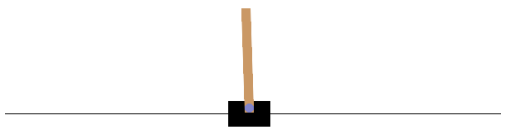
\includegraphics[width=.8\linewidth]{images/cart-pole.png}
    \captionof{figure}{Random observed environment state.}
    \label{fig:cart-pole}
\end{minipage}

\vspace{0.2cm}

The cart–pole environment (seen in Figure \ref{fig:cart-pole}) is a part of the \textit{Gymnasium} package in python. This package contains a number of different virtual environments which can be imported and used to train and validate ones own reinforcement agents. \cite{Gymnasium} \cite{Cart-pole}

\vspace{0.2cm}

\begin{lstlisting}
    import gymnasium as gym

    environment = gym.make('CartPole-v1', render_mode="rgb_array")
    state, _ = environment.reset()
\end{lstlisting}

The agent controls the cart movement, \textit{i.e.}, by pushing it one way or another. The termination (or truncation) is determined by the observed values, or if the episode length is greater than $500$ time–steps. For every time–step until termination or truncation, the agent is given a reward of $+1$.

\vspace{0.3cm}

\begin{tabular}{ccc}
    \begin{tabular}{llll}
        & \textbf{OBSERVATIONS} & \textbf{VALUES} \\ \\
        $x$ & cart position & $0 \rightarrow \pm 2.4$ \\
        $\Vec{v}$ & cart velocity & $0 \rightarrow \pm \infty$ \\
        $\theta$ & pole angle & $0 \rightarrow \pm 12^\circ$ \\
        $\Vec{\omega}$ & pole angular velocity & $0 \rightarrow \pm \infty$ \\
    \end{tabular}
    &
    \begin{tabular}{ll}
        & \textbf{ACTIONS} \\ \\
        0 & push cart to the left \\
        1 & push cart to the right \\
        & \\
        & \\
    \end{tabular}
    &
    \begin{tabular}{ll}
        & \textbf{REWARDS} \\ \\
        $+1$ & every time–step \\
        & (until termination) \\
        & \\
        & \\
    \end{tabular}
\end{tabular}

\subsection*{Policy–based gradient agent}
\begin{leftbar}
    Initialising the policy–based agent with four inputs and two outputs, with $15$ and $30$ nodes in the hidden layers, and training it during $10 000$ games of play and self–improvement led to surprisingly good results. The agent was trained with the \textit{RMSprop} optimizer with a learning–rate of $0.00025$ and a reward discount of $0.99$. See Figure \ref{fig:policy-based-metrics} in the \hyperlink{sec:results}{results}.
\end{leftbar}
\subsection*{Value–based Q–learning agent}
\begin{leftbar}
    Likewise, the value–based agent was initialised with the same hyper-parameters as the policy–based agent, only scaling the learning–rate by a factor of ten due to using mini–batches.

    In addition, the Q–learning agent had a $\gamma$–value of $0.99$ and respectively exploration rate, decay and minimum values of $1$, $0.995$ and $0.01$.

    The agent was trained during $5 000$ games using the mentioned \hyperlink{alg:dqn}{algorithm}. The agent had a memory of $1 500$ games and was updated with $64$ game sequences every ten games it played. The target network, $\Hat{Q}$ was updated every $250$ games. See Figure \ref{fig:value-based-metrics} in the \hyperlink{sec:results}{results}.
\end{leftbar}

\hypertarget{seq:tetris}{}
\section*{Tetris environment}

\newpage
\printbibliography

\newpage
\hypertarget{sec:results}{}
\section*{Results}

\begin{figure}[h]
    \centering
    \begin{minipage}{0.5\textwidth}
        \centering
        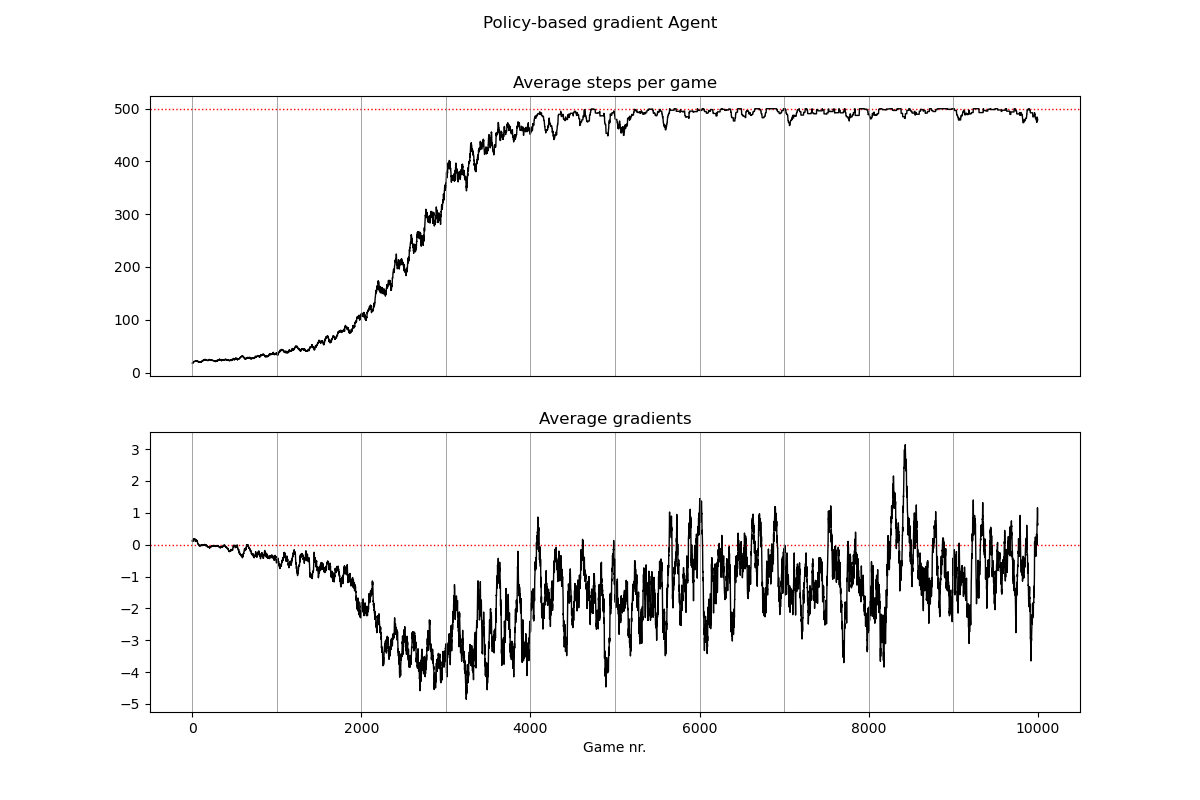
\includegraphics[width=\linewidth]{images/torch-pbg.png}
        \caption{Training of the policy–based agent.}
        \label{fig:policy-based-metrics}
    \end{minipage}\hfill
    \begin{minipage}{0.5\textwidth}
        \centering
        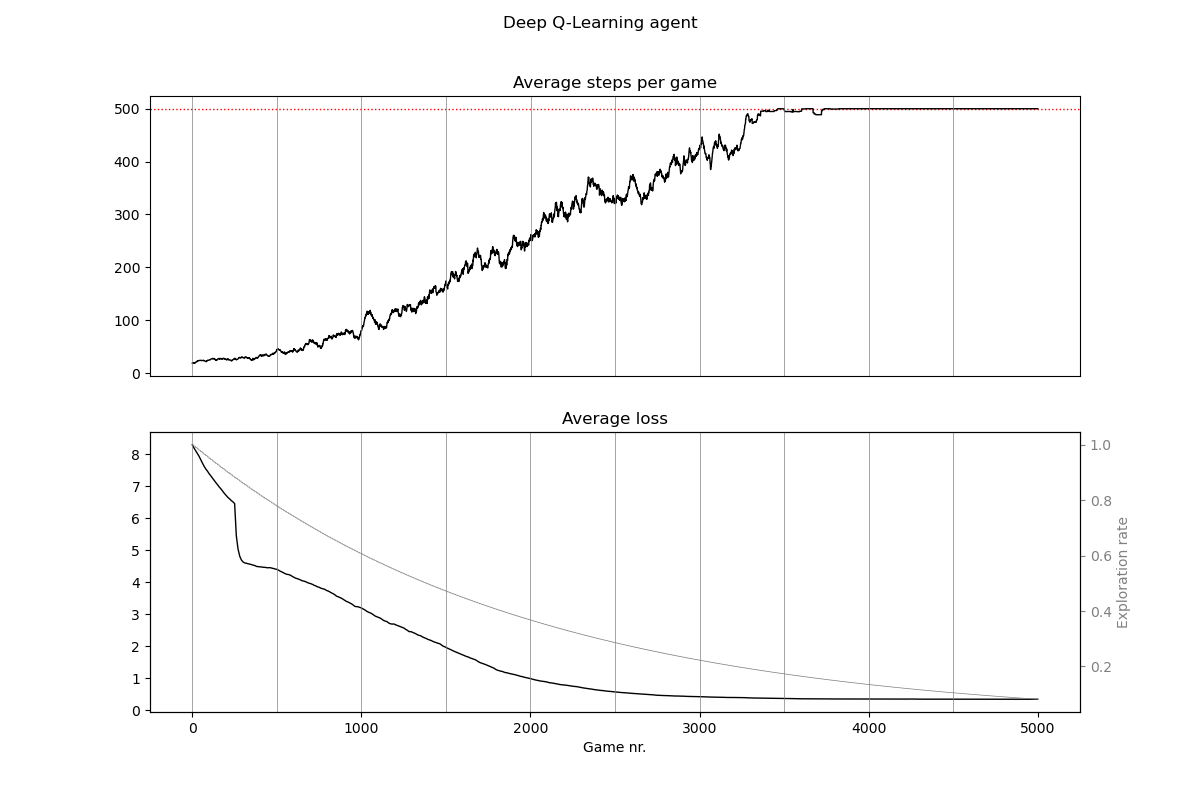
\includegraphics[width=\linewidth]{images/torch-dqn.png}
        \caption{Training of the value–based (DQN) agent.}
        \label{fig:value-based-metrics}
    \end{minipage}
\end{figure}

\newpage
\hypertarget{sec:code}{}
\section*{Code}

\end{document}
